This document describes the solution to the \textbf{Academy Re-Win -- Entrance Challenge}, the admission challenge of Gecko Academy (Binary Gecko). The challenge is a single Windows binary with \textbf{four chained reverse-engineering levels}: each level unlocks only after the previous one is solved, and the difficulty grows from a classic keygen up to a virtual machine with its own bytecode.

The goal of each level is not to guess a password but to \textbf{understand the validation algorithm} from the disassembled code and reproduce it, so that a valid credential can be generated for any input.

\subsection{Challenge structure}

\begin{table}[H]
\centering
\rowcolors{2}{TableBgRowColor}{TableBgRowIntemediaColor}
\begin{tabularx}{\linewidth}{c l X l}
\rowcolor{TableHeaderBgRowColor}
\textcolor{white}{\textbf{Level}} & \textcolor{white}{\textbf{Difficulty}} & \textcolor{white}{\textbf{What is asked}} & \textcolor{white}{\textbf{Status}} \\
1 & Medium & Username and an 8-hex-digit serial derived from it (keygen). & Solved \\
2 & -- & Serial in the format \texttt{XXXX-XXXX-XXXX-YYYY}, computed from the Level 1 username. & Solved \\
3 & Hard & Login: freely chosen username (at least 5 characters) and its password. & Solved \\
4 & Very hard & Password validated by an internal virtual machine; its bytecode must be understood. & Pending \\
\end{tabularx}
\caption{Levels of the Academy Re-Win Entrance Challenge}
\end{table}

\subsection{Results}

Figure~\ref{fig:levels} shows the challenge running with the generated credentials: Levels 1 to 3 pass and the binary unlocks the final level.

\begin{table}[H]
\centering
\rowcolors{2}{TableBgRowColor}{TableBgRowIntemediaColor}
\begin{tabularx}{\linewidth}{c X X}
\rowcolor{TableHeaderBgRowColor}
\textcolor{white}{\textbf{Level}} & \textcolor{white}{\textbf{Input}} & \textcolor{white}{\textbf{Valid credential}} \\
1 & Username: \texttt{mati} & Serial: \texttt{00389E38} \\
2 & Username: \texttt{mati} (inherited) & Serial: \texttt{E834-69B6-1B27-9AA5} \\
3 & Username: \texttt{fierro} & Password: \texttt{C65715F2BE5918C4} \\
4 & -- & \emph{Under analysis} \\
\end{tabularx}
\caption{Generated valid credentials}
\end{table}

\begin{figure}[H]
\centering
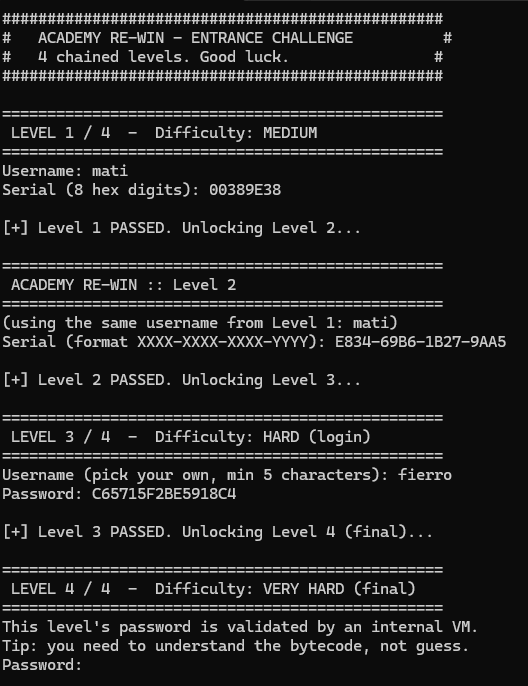
\includegraphics[width=0.55\linewidth]{initial/img/levels.png}
\caption{Challenge run: Levels 1 to 3 passed}
\label{fig:levels}
\end{figure}

\subsection{Methodology and tools}

The same process was followed for every level:

\begin{enumerate}
    \item \textbf{Reconnaissance:} run the binary and observe its messages and expected input format.
    \item \textbf{Static analysis:} locate the validation routine in the disassembler from strings and I/O calls.
    \item \textbf{Dynamic analysis:} confirm the behaviour in a debugger with breakpoints on the final comparison.
    \item \textbf{Algorithm reconstruction:} rewrite the validation in a high-level language.
    \item \textbf{Keygen and verification:} generate credentials for arbitrary usernames and check them against the binary.
\end{enumerate}

% TODO: adjust the tool list to the ones actually used
Tools used: \emph{Ghidra / IDA} (static analysis), \emph{x64dbg} (dynamic analysis) and \emph{Python} (keygens).
